\documentclass[conference]{IEEEtran}
\IEEEoverridecommandlockouts
% The preceding line is only needed to identify funding in the first footnote.
\usepackage{cite}
\usepackage{amsmath,amssymb,amsfonts}
\usepackage{algorithmic}
\usepackage{graphicx}
\usepackage{textcomp}
\usepackage{xcolor}
\usepackage{booktabs}
\usepackage{array}
\usepackage{url}
\usepackage{tikz}
\usepackage{float}
\usetikzlibrary{arrows.meta,positioning,shapes.geometric,fit}

\setlength{\textfloatsep}{8pt plus 1pt minus 2pt}
\setlength{\floatsep}{6pt plus 1pt minus 2pt}
\setlength{\intextsep}{6pt plus 1pt minus 2pt}
\setlength{\abovecaptionskip}{4pt}
\setlength{\belowcaptionskip}{0pt}
\def\BibTeX{{\rm B\kern-.05em{\sc i\kern-.025em b}\kern-.08em
    T\kern-.1667em\lower.7ex\hbox{E}\kern-.125emX}}

\title{Securing Open-Source Supply Chains Through Automated Dependency Vulnerability Analysis\\
\thanks{This work did not receive external funding.}}

\author{
\IEEEauthorblockN{Sara Gorule}
\IEEEauthorblockA{\textit{Department of Computer Engineering} \\
\textit{Vidyavardhini's College of Engineering}\\
and Technology\\
Vasai, India \\
sara.231423201@vcet.edu.in}
\and
\IEEEauthorblockN{Smit Barve}
\IEEEauthorblockA{\textit{Department of Computer Engineering} \\
\textit{Vidyavardhini's College of Engineering}\\
and Technology\\
Vasai, India \\
smit.231033105@vcet.edu.in}
\and
\IEEEauthorblockN{Yashasvi Chunchu}
\IEEEauthorblockA{\textit{Department of Computer Engineering} \\
\textit{Vidyavardhini's College of Engineering}\\
and Technology\\
Vasai, India \\
yashasvi.231253201@vcet.edu.in}
\and
\IEEEauthorblockN{Riddhi Churi}
\IEEEauthorblockA{\textit{Department of Computer Engineering} \\
\textit{Vidyavardhini's College of Engineering}\\
and Technology\\
Vasai, India \\
Riddhi.231273201@vcet.edu.in}
\and
\IEEEauthorblockN{Prof. Swati Verma}
\IEEEauthorblockA{\textit{Department of Computer Engineering} \\
\textit{Vidyavardhini's College of Engineering}\\
and Technology\\
Vasai, India \\
swati.verma@vcet.edu.in}
\and
\IEEEauthorblockN{Dr. Megha Trivedi}
\IEEEauthorblockA{\textit{Department of Computer Engineering} \\
\textit{Vidyavardhini's College of Engineering}\\
and Technology\\
Vasai, India \\
megha.trivedi@vcet.edu.in}
}

\begin{document}
\raggedbottom
\maketitle

\begin{abstract}
Open-source software reuse has become fundamental to modern software engineering, but it has also expanded the attack surface of software supply chains. Vulnerabilities in direct and transitive dependencies, accidental secret exposure, and malicious code injection increasingly affect downstream repositories and CI pipelines. This paper presents VulnAI, a GitHub-native framework for automated dependency and repository risk analysis at push time. VulnAI combines dependency vulnerability lookup, change-aware repository scanning, secret and risky-code detection, malicious-pattern identification, and owner-aware reporting to produce actionable security digests for maintainers. In addition to the deterministic pipeline, we evaluate a compact deep learning extension for malicious and obfuscated code triage on an expanded public PyPI benchmark slice derived from real malicious packages. The system is informed by prior research on secret leakage in GitHub repositories, propagated vulnerabilities in reused components, commit-level vulnerability detection, and learning-based code security analysis. Rather than replacing deterministic analysis with opaque models, VulnAI uses a practical layered design that supports lightweight deployment today while remaining compatible with future model-based enrichment. This paper describes the motivation, literature grounding, architecture, workflow, benchmark methodology, and design rationale of the framework.
\end{abstract}

\begin{IEEEkeywords}
software supply chain security, open-source dependencies, vulnerability detection, secret scanning, malicious code detection, repository security, GitHub Actions
\end{IEEEkeywords}

\section{Introduction}
\subsection{Background and Motivation}
Open-source dependencies now form a critical part of nearly every software system. This reuse accelerates development, but it also causes downstream projects to inherit weaknesses from external packages, libraries, and transitive components. Security problems in repositories are not limited to dependency CVEs alone; they also include secret leakage, unsafe code patterns, accidental state exposure, and malicious code insertion.

Prior work shows that repository-level security exposure is widespread. Meli \emph{et al.} performed a large-scale longitudinal study of public GitHub repositories and found that secret leakage affected over 100{,}000 repositories, with thousands of new unique secrets leaked daily~\cite{meli2019how}. In parallel, research on reused open-source components shows that vulnerable code often propagates into downstream software in modified form, making simple version-based detection insufficient~\cite{woo2022movery,woo2023v1scan}. These results motivate automated, repository-integrated analysis that can operate continuously and present findings in a form that maintainers can act on quickly.

\subsection{Problem Statement}
Existing security tools often focus on isolated categories such as software composition analysis, secret scanning, or static code analysis. In practice, maintainers need an integrated system that answers a more operational question: what risky artifact or vulnerable dependency was introduced in the current push, where is it located, and who should respond first. Tools that surface only raw matches or package advisories often generate noise without enough context for fast remediation.

\subsection{Objectives and Contributions}
The primary objectives of VulnAI are:
\begin{itemize}
\item Detect vulnerabilities in open-source dependencies through automated lockfile and manifest analysis.
\item Identify repository-level risks such as committed secrets, risky APIs, suspicious code paths, and memory or state artifacts.
\item Prioritize findings based on whether they are newly introduced in the current push.
\item Route findings toward probable maintainers using \texttt{CODEOWNERS}-style ownership metadata.
\item Produce lightweight CI-ready reports that can be integrated into GitHub-native workflows.
\end{itemize}

The current scope of VulnAI focuses on GitHub-centered repository scanning and dependency analysis within CI. The implemented framework emphasizes deterministic detection and operational reporting rather than exploitability proof. The main contributions of this work are a push-time repository security framework, an owner-aware reporting workflow, and an experimental deep learning extension for malicious and obfuscated code triage on a public PyPI benchmark slice.

\begin{figure}[htbp]
\centering
\resizebox{\columnwidth}{!}{%
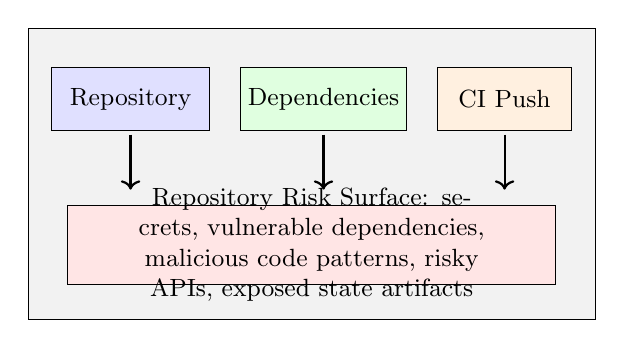
\begin{tikzpicture}[font=\small]
\draw[fill=gray!10,draw=black] (0,0) rectangle (7.2,3.7);
\draw[fill=blue!12,draw=black] (0.3,2.4) rectangle (2.3,3.2);
\node at (1.3,2.8) {Repository};
\draw[fill=green!12,draw=black] (2.7,2.4) rectangle (4.8,3.2);
\node at (3.75,2.8) {Dependencies};
\draw[fill=orange!12,draw=black] (5.2,2.4) rectangle (6.9,3.2);
\node at (6.05,2.8) {CI Push};
\draw[->,thick] (1.3,2.35) -- (1.3,1.65);
\draw[->,thick] (3.75,2.35) -- (3.75,1.65);
\draw[->,thick] (6.05,2.35) -- (6.05,1.65);
\draw[fill=red!10,draw=black] (0.5,0.45) rectangle (6.7,1.45);
\node[align=center,text width=5.7cm] at (3.6,0.95) {Repository Risk Surface: secrets, vulnerable dependencies, malicious code patterns, risky APIs, exposed state artifacts};
\end{tikzpicture}
}
\caption{Conceptual repository and dependency risk surface addressed by VulnAI.}
\label{fig:risk_surface}
\end{figure}

Fig.~\ref{fig:risk_surface} highlights the paper's central problem framing: repository events, dependency state, and CI activity all feed into a shared risk surface in which secrets, vulnerable packages, risky APIs, malicious logic, and exposed state artifacts can appear together and must therefore be analyzed as a combined security problem rather than as isolated checks.

\section{Literature Review}
\subsection{Open-Source Supply Chain Security}
Secret leakage remains one of the most persistent repository security failures. Meli \emph{et al.} demonstrate that large-scale secret exposure on GitHub is systemic rather than anecdotal and that high-confidence detection requires conservative validation rather than naive entropy matching alone~\cite{meli2019how}. This directly supports VulnAI's use of structured secret patterns and artifact-focused scanning.

\subsection{Malicious and Obfuscated Code Detection}
MOVERY studies modified vulnerable code clone discovery and shows that downstream reused code frequently differs syntactically from the original vulnerable source, which makes exact matching unreliable~\cite{woo2022movery}. V1SCAN extends this line of work by combining version-based and code-based classification techniques to discover one-day vulnerabilities in reused C/C++ components~\cite{woo2023v1scan}. These findings support the need for dependency-aware analysis that goes beyond simplistic package presence checks.

\subsection{Deep Learning for Code Analysis}
Recent work such as ChainFuzz emphasizes that software composition analysis may flag large numbers of upstream vulnerabilities without proving exploitability in downstream software~\cite{deng2025chainfuzz}. Their results show that downstream validation is difficult because custom code, cross-layer constraints, and transitive dependencies change the triggering conditions of vulnerabilities. This motivates VulnAI's design choice to treat dependency alerts as actionable triage signals, not as final proof of exploitability.

\subsection{Research Gap}
Commit-level vulnerability analysis is especially relevant for CI-integrated security. Li \emph{et al.} propose neural commit-level vulnerability detection and assessment, including extensions to fine-grained CWE-type prediction~\cite{li2023commit}. In the learning-based setting, VulBERTa demonstrates that pre-trained source-code models can achieve strong vulnerability detection performance~\cite{hanif2022vulberta}, and MSIVD shows that combining code, vulnerability explanations, and graph structure can improve LLM-based detection~\cite{yang2024msivd}. A recent systematic literature review by Kaniewski \emph{et al.} synthesizes 263 studies on LLM-based software vulnerability detection and emphasizes the current fragmentation in system designs, dataset usage, and evaluation methodology~\cite{kaniewski2025slr}. VulnAI adopts the operational lessons from this literature while keeping its current implementation deterministic.

\noindent Existing work tends to focus on either supply-chain advisories, malicious-package detection, or learning-based code understanding in isolation. VulnAI is motivated by the gap between these strands: maintainers need a lightweight system that can integrate dependency analysis, suspicious-code triage, and reporting directly into repository workflows.

Tsfaty and Fire propose MSDT, an anomaly-based method for malicious source code detection in open-source packages, and show that representation learning can help identify injected malicious functions~\cite{tsfaty2023malicious}. Their study uses a dataset of 607{,}461 functions and reports precision@k values of up to 0.909 for malicious code injection detection~\cite{tsfaty2023malicious}. This motivates the inclusion of a malicious-code lens in VulnAI for downloader chains, encoded execution, exfiltration patterns, and persistence-oriented behavior.

\begin{table}[htbp]
\caption{Research Themes and Their Influence on VulnAI}
\label{tab:litmap}
\centering
\renewcommand{\arraystretch}{1.2}
\begin{tabular}{p{2.0cm}p{2.15cm}p{2.8cm}}
\toprule
\textbf{Theme} & \textbf{Representative Work} & \textbf{Influence on VulnAI} \\
\midrule
Secret exposure & Meli et al.~\cite{meli2019how} & Conservative secret and artifact detection \\
Reused vulnerability discovery & MOVERY, V1SCAN~\cite{woo2022movery,woo2023v1scan} & Dependency-aware triage and modified-code awareness \\
Exploitability validation & ChainFuzz~\cite{deng2025chainfuzz} & Treat SCA hits as signals, not proof \\
Commit-level security analysis & Li et al.~\cite{li2023commit} & Change-aware prioritization in CI \\
Learning-based vulnerability detection & VulBERTa, MSIVD~\cite{hanif2022vulberta,yang2024msivd} & Future path for enrichment and ranking \\
LLM survey evidence & Kaniewski et al.~\cite{kaniewski2025slr} & Cautious positioning of LLMs as optional enrichment \\
Malicious source-code analysis & Tsfaty and Fire~\cite{tsfaty2023malicious} & Backdoor and exfiltration pattern lens \\
\bottomrule
\end{tabular}
\end{table}

\section{Proposed System}
\subsection{System Overview}
VulnAI is designed as a GitHub-native push-time scanning framework. The architecture is divided into five major functional layers:
\begin{itemize}
\item repository context collection,
\item deterministic content analysis,
\item dependency vulnerability enrichment,
\item ownership-aware report generation, and
\item notification and CI response.
\end{itemize}

The system operates on each push and aims to convert repository events into a compact risk digest for maintainers.

\begin{figure}[htbp]
\centering
\resizebox{\columnwidth}{!}{%
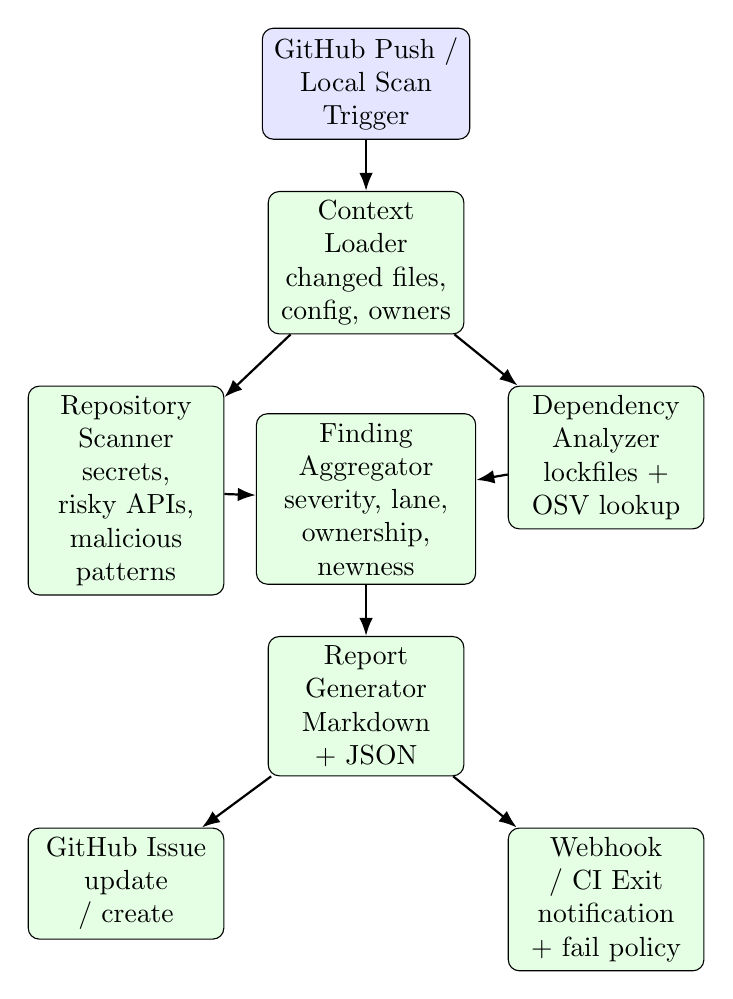
\begin{tikzpicture}[
node distance=0.65cm and 0.45cm,
box/.style={draw, rounded corners, text width=2.4cm, minimum height=0.9cm, align=center, fill=blue!10},
smallbox/.style={draw, rounded corners, text width=2.25cm, minimum height=0.8cm, align=center, fill=green!10},
arrow/.style={-{Latex[length=2.3mm]}, thick}
]
\node[box] (push) {GitHub Push /\\ Local Scan Trigger};
\node[smallbox, below=of push] (context) {Context Loader\\ changed files, config, owners};
\node[smallbox, below left=of context, xshift=-0.1cm] (repo) {Repository Scanner\\ secrets, risky APIs,\\ malicious patterns};
\node[smallbox, below right=of context, xshift=0.1cm] (dep) {Dependency Analyzer\\ lockfiles + OSV lookup};
\node[smallbox, below=1.0cm of context, text width=2.55cm] (merge) {Finding Aggregator\\ severity, lane, ownership, newness};
\node[smallbox, below=of merge] (report) {Report Generator\\ Markdown + JSON};
\node[smallbox, below left=of report, xshift=-0.1cm] (issue) {GitHub Issue\\ update / create};
\node[smallbox, below right=of report, xshift=0.1cm] (webhook) {Webhook / CI Exit\\ notification + fail policy};
\draw[arrow] (push) -- (context);
\draw[arrow] (context) -- (repo);
\draw[arrow] (context) -- (dep);
\draw[arrow] (repo) -- (merge);
\draw[arrow] (dep) -- (merge);
\draw[arrow] (merge) -- (report);
\draw[arrow] (report) -- (issue);
\draw[arrow] (report) -- (webhook);
\end{tikzpicture}
}
\caption{VulnAI architecture and push-time analysis pipeline.}
\label{fig:architecture}
\end{figure}

As shown in Fig.~\ref{fig:architecture}, the system starts from a push or local scan trigger, gathers repository context, runs repository and dependency analysis in parallel, merges the resulting findings into a normalized structure, and then emits reports or enforcement actions through issues, webhooks, and CI exit behavior.

\subsection{System Architecture}
VulnAI first collects repository context, including configuration, the set of files modified in the current push, and ownership rules derived from \texttt{CODEOWNERS}. This stage enables the system to distinguish newly introduced findings from pre-existing repository debt.

\subsection{Dependency Analysis}
VulnAI parses dependency manifests and lockfiles, extracts package coordinates, and queries OSV for known vulnerabilities. The goal is to provide actionable supply-chain awareness with low operational overhead. Because dependency advisories do not by themselves establish reachability or exploitability~\cite{deng2025chainfuzz}, findings are framed as prioritized risk indicators rather than definitive exploitability claims.

\subsection{Malicious Code Detection}
The deterministic scanning layer analyzes repository files for:
\begin{itemize}
\item structured secrets such as private keys and cloud credentials,
\item risky code primitives such as \texttt{eval}, shell execution, or unsafe deserialization,
\item malicious or backdoor-like behavior patterns including downloader chains and exfiltration,
\item memory and state artifacts such as \texttt{.env}, logs, sessions, and transcript-like files.
\end{itemize}

This layer emphasizes transparent rules and lightweight execution, which is appropriate for CI deployment and reviewer trust.

\subsection{Obfuscated Code Detection}
Beyond explicit malicious patterns, VulnAI also targets encoded payloads, hidden execution chains, staged decoding behavior, and related obfuscation markers. This is especially important for malicious packages that conceal intent behind string reconstruction, base64 decoding, downloader stubs, or delayed execution.

\subsection{Reporting and Integration}
All findings are normalized into a common structure containing path, severity, summary, remediation text, tags, ownership, and whether the finding is newly introduced. VulnAI then renders the results into Markdown and JSON for both human review and downstream tooling. The final layer supports GitHub issue updates, webhook notifications, and CI failure thresholds. This makes VulnAI suitable both as a passive reporting system and as an active enforcement mechanism when configured conservatively.

\begin{table}[htbp]
\caption{VulnAI Detection Categories}
\label{tab:categories}
\centering
\renewcommand{\arraystretch}{1.2}
\begin{tabular}{p{1.75cm}p{1.6cm}p{3.45cm}}
\toprule
\textbf{Category} & \textbf{Examples} & \textbf{Purpose} \\
\midrule
Secret & AWS keys, PATs, private keys & prevent credential exposure \\
Risky code & \texttt{eval}, \texttt{exec}, unsafe deserialization & flag insecure implementation patterns \\
Malicious code & downloader chains, exfiltration, persistence hooks & surface likely backdoor behavior \\
State artifacts & logs, sessions, transcripts, \texttt{.env} files & reduce privacy and runtime-state leakage \\
Dependency CVE & vulnerable locked packages & identify supply-chain weakness \\
\bottomrule
\end{tabular}
\end{table}

\paragraph{Learning-Based Extension for Malicious Package Triage.}
Beyond the deterministic scanner, we implemented a compact sequence model for classifying code snippets as benign or malicious while also predicting whether obfuscation is present. The goal of this extension is not to replace VulnAI's rule-based controls, but to enrich suspicious-code triage when repositories or package artifacts contain encoded payloads, downloader chains, or behavior that is difficult to summarize with a single deterministic rule.

\begin{figure}[htbp]
\centering
\resizebox{0.36\columnwidth}{!}{%
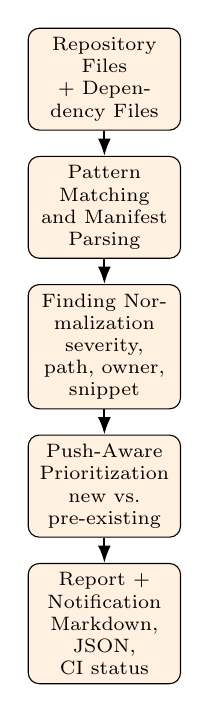
\begin{tikzpicture}[
font=\scriptsize,
node distance=0.32cm,
proc/.style={draw, rounded corners, text width=1.7cm, minimum height=0.56cm, align=center, fill=orange!12},
arrow/.style={-{Latex[length=2.2mm]}, thick}
]
\node[proc] (a) {Repository Files\\ + Dependency Files};
\node[proc, below=of a] (b) {Pattern Matching\\ and Manifest Parsing};
\node[proc, below=of b] (c) {Finding Normalization\\ severity, path, owner, snippet};
\node[proc, below=of c] (d) {Push-Aware Prioritization\\ new vs. pre-existing};
\node[proc, below=of d] (e) {Report + Notification\\ Markdown, JSON, CI status};
\draw[arrow] (a) -- (b);
\draw[arrow] (b) -- (c);
\draw[arrow] (c) -- (d);
\draw[arrow] (d) -- (e);
\end{tikzpicture}
}
\caption{Detection and reporting workflow used by the framework.}
\label{fig:workflow}
\end{figure}

Fig.~\ref{fig:workflow} compresses the operational path into a linear flow: input files are scanned and parsed, raw detections are normalized, new findings are separated from pre-existing debt, and the final output is converted into human-readable and machine-readable reporting artifacts.

\begin{table}[htbp]
\caption{Core Modules of the VulnAI Framework}
\label{tab:modules}
\centering
\renewcommand{\arraystretch}{1.2}
\begin{tabular}{p{2.1cm}p{1.65cm}p{3.05cm}}
\toprule
\textbf{Module} & \textbf{Input} & \textbf{Output} \\
\midrule
Context loader & push metadata, config, ownership rules & changed-file set, scan context \\
Repository scanner & tracked files & repository findings with snippets \\
Dependency analyzer & lockfiles, manifests & dependency CVE findings \\
Aggregator & raw findings & normalized finding objects \\
Reporter & normalized findings & Markdown and JSON reports \\
Notifier & reports, tokens, webhook URL & issue updates, webhook payloads, CI result \\
\bottomrule
\end{tabular}
\end{table}

\section{Dataset and Methodology}
\subsection{Dataset Sources}
The experimental detector was evaluated on an expanded public PyPI benchmark slice constructed from two sources. The malicious side was derived from a local copy of the \texttt{pypi-malregistry} corpus, which contains real malicious package artifacts collected from the PyPI ecosystem. The benign side was built from installed Python package files used as non-malicious controls. This produced a balanced dataset with equal numbers of malicious and benign code samples at the corpus level.

\subsection{Data Preparation}
Package archives were parsed to extract Python and related source files, after which suspicious-code samples were retained from malicious packages and paired with benign package code from the control set. Each sample was normalized into a common JSONL format containing language, code content, and labels. The final split contained 640 training examples and 160 held-out evaluation examples, with both malicious and benign samples represented in each split.

\subsection{Model Architecture}
The best-performing learning-based model is a compact bidirectional GRU classifier over code-token sequences. Input snippets are tokenized, embedded, and passed through a two-layer bidirectional GRU encoder. Mean pooling and max pooling are then applied over the encoded sequence, and the pooled representation is used by two linear heads: one for verdict classification and one for obfuscation prediction. Fig.~\ref{fig:model_architecture} summarizes both the bidirectional token-flow view and the exact PyTorch layer stack used in the implementation.

\begin{figure}[htbp]
\centering
\resizebox{0.84\columnwidth}{!}{%
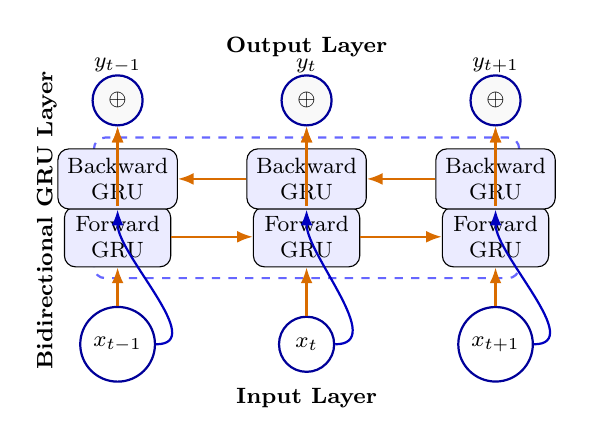
\begin{tikzpicture}[
font=\footnotesize,
x=1.2cm,y=1.05cm,
node/.style={circle, draw=blue!60!black, thick, minimum size=7mm, fill=white},
gru/.style={draw, rectangle, rounded corners, minimum width=1.35cm, minimum height=0.7cm, align=center, fill=blue!8},
op/.style={circle, draw=blue!60!black, thick, minimum size=6mm, fill=gray!5},
box/.style={draw=blue!60, dashed, rounded corners, thick},
arr/.style={-{Latex[length=2mm]}, thick, orange!85!black},
guide/.style={-{Latex[length=2mm]}, thick, blue!75!black}
]
\node at (2,2.65) {\textbf{Output Layer}};
\node at (2,-1.6) {\textbf{Input Layer}};
\node[rotate=90] at (-0.75,0.55) {\textbf{Bidirectional GRU Layer}};
\draw[box] (-0.25,-0.15) rectangle (4.25,1.55);
\foreach \x/\lbl in {0/$x_{t-1}$,2/$x_t$,4/$x_{t+1}$} {\node[node] (in\x) at (\x,-0.95) {\lbl};}
\foreach \x/\lbl in {0/$y_{t-1}$,2/$y_t$,4/$y_{t+1}$} {\node[op] (out\x) at (\x,2.0) {$\oplus$}; \node at (\x,2.42) {\lbl};}
\node[gru] (f0) at (0,0.35) {Forward\\GRU};
\node[gru] (f2) at (2,0.35) {Forward\\GRU};
\node[gru] (f4) at (4,0.35) {Forward\\GRU};
\node[gru] (b0) at (0,1.05) {Backward\\GRU};
\node[gru] (b2) at (2,1.05) {Backward\\GRU};
\node[gru] (b4) at (4,1.05) {Backward\\GRU};
\draw[arr] (in0) -- (f0);
\draw[arr] (in2) -- (f2);
\draw[arr] (in4) -- (f4);
\draw[arr] (b0) -- (out0);
\draw[arr] (b2) -- (out2);
\draw[arr] (b4) -- (out4);
\draw[arr] (f0) -- (out0);
\draw[arr] (f2) -- (out2);
\draw[arr] (f4) -- (out4);
\draw[arr] (f0.east) -- (f2.west);
\draw[arr] (f2.east) -- (f4.west);
\draw[arr] (b4.west) -- (b2.east);
\draw[arr] (b2.west) -- (b0.east);
\draw[guide] (in0.east) .. controls +(0.55,0) and +(0,-0.55) .. (b0.south);
\draw[guide] (in2.east) .. controls +(0.55,0) and +(0,-0.55) .. (b2.south);
\draw[guide] (in4.east) .. controls +(0.55,0) and +(0,-0.55) .. (b4.south);
\end{tikzpicture}
}
\vspace{0.25em}
\resizebox{0.84\columnwidth}{!}{%
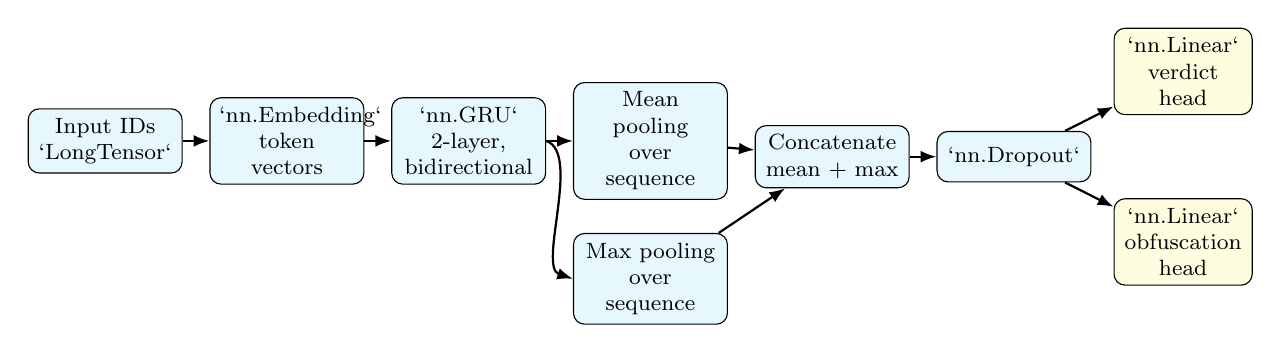
\begin{tikzpicture}[
font=\footnotesize,
node distance=0.42cm and 0.34cm,
layer/.style={draw, rounded corners, text width=1.72cm, minimum height=0.64cm, align=center, fill=cyan!10},
head/.style={draw, rounded corners, text width=1.52cm, minimum height=0.62cm, align=center, fill=yellow!12},
arr/.style={-{Latex[length=2mm]}, thick}
]
\node[layer] (input) {Input IDs\\`LongTensor`};
\node[layer, right=of input] (embed) {`nn.Embedding`\\token vectors};
\node[layer, right=of embed] (gru) {`nn.GRU`\\2-layer, bidirectional};
\node[layer, right=of gru] (avg) {Mean pooling\\over sequence};
\node[layer, below=of avg] (max) {Max pooling\\over sequence};
\node[layer, right=of avg, yshift=-0.2cm] (concat) {Concatenate\\mean + max};
\node[layer, right=of concat] (drop) {`nn.Dropout`};
\node[head, above right=0.2cm and 0.28cm of drop] (verdict) {`nn.Linear`\\verdict head};
\node[head, below right=0.2cm and 0.28cm of drop] (obf) {`nn.Linear`\\obfuscation head};
\draw[arr] (input) -- (embed);
\draw[arr] (embed) -- (gru);
\draw[arr] (gru) -- (avg);
\draw[arr] (gru.east) .. controls +(0.45,-0.15) and +(-0.45,0.15) .. (max.west);
\draw[arr] (avg) -- (concat);
\draw[arr] (max) -- (concat);
\draw[arr] (concat) -- (drop);
\draw[arr] (drop) -- (verdict);
\draw[arr] (drop) -- (obf);
\end{tikzpicture}
}
\caption{Best-performing BiGRU detector: top, bidirectional token-context flow; bottom, PyTorch layer stack used in the VulnAI experiments.}
\label{fig:model_architecture}
\end{figure}

The upper half of Fig.~\ref{fig:model_architecture} illustrates how forward and backward GRU passes capture token context from both directions before combining the hidden states, while the lower half maps that idea to the implemented stack of embedding, bidirectional recurrent encoding, pooled sequence summaries, dropout, and task-specific output heads.

\subsection{Training Setup}
Training was performed on the 640-example training split using compact non-LLM architectures, including BiGRU and hybrid Transformer-CNN variants. The strongest result came from a widened BiGRU configuration with an expanded vocabulary, longer context window, and stronger hidden-state capacity. The training objective jointly optimized verdict classification and obfuscation prediction so that the model could learn both malicious intent and concealment-related signals.

\begin{table}[htbp]
\caption{Expanded Public PyPI Benchmark Slice Used in This Work}
\label{tab:dataset}
\centering
\renewcommand{\arraystretch}{1.2}
\begin{tabular}{p{2.2cm}p{1.2cm}p{1.2cm}p{1.45cm}}
\toprule
\textbf{Split} & \textbf{Total} & \textbf{Malicious} & \textbf{Benign} \\
\midrule
Training & 640 & 326 & 314 \\
Evaluation & 160 & 74 & 86 \\
Overall & 800 & 400 & 400 \\
\bottomrule
\end{tabular}
\end{table}

\subsection{Evaluation Metrics}
We report verdict accuracy, malicious recall, and obfuscation accuracy on the 160-example held-out split. These metrics were chosen to capture both overall classification quality and the model's ability to detect malicious or concealed code. The benchmark is intentionally larger and less fragile than the earlier pilot slice of 27 examples. However, it is still not identical to MalwareBench or the datasets used by PyPIGuard, DySec, or One Detector Fits All. Therefore, comparisons against published systems should be interpreted as cross-study reference points rather than same-split head-to-head results.

\section{Results and Discussion}
\subsection{Experimental Results}
Table~\ref{tab:internal_results} and Fig.~\ref{fig:accuracy_chart} summarize the performance of the rule baseline and the compact deep learning variants on the expanded benchmark. The widened BiGRU and hybrid models substantially outperform the deterministic baseline, while the BiGRU wide configuration achieves the best overall balance between accuracy and malicious recall.

\begin{table}[htbp]
\caption{Internal Model Comparison on the Expanded PyPI Benchmark}
\label{tab:internal_results}
\centering
\renewcommand{\arraystretch}{1.2}
\begin{tabular}{p{2.3cm}p{1.25cm}p{1.35cm}p{1.2cm}}
\toprule
\textbf{Model} & \textbf{Accuracy} & \textbf{Malicious Recall} & \textbf{Obf. Acc.} \\
\midrule
Rule baseline & 85.00\% & 67.57\% & -- \\
Hybrid baseline & 96.88\% & 100.00\% & 96.25\% \\
BiGRU baseline & 98.13\% & 98.65\% & 96.88\% \\
Hybrid wide & 98.75\% & 98.65\% & 98.13\% \\
\textbf{BiGRU wide} & \textbf{98.75\%} & \textbf{100.00\%} & 96.88\% \\
\bottomrule
\end{tabular}
\end{table}

\begin{figure}[htbp]
\centering
\resizebox{\columnwidth}{!}{%
\begin{tikzpicture}[x=0.62cm,y=0.055cm,font=\scriptsize]
\draw[->] (0,0) -- (10.2,0);
\draw[->] (0,0) -- (0,105);
\foreach \y in {0,20,40,60,80,100} {
  \draw (0,\y) -- (-0.12,\y);
  \node[left] at (0,\y) {\y};
}
\foreach \x/\name/\val/\color in {
  1/{Rule}/85/{gray!55},
  3/{Hybrid\\ base}/96.88/{blue!35},
  5/{BiGRU\\ base}/98.13/{green!45},
  7/{Hybrid\\ wide}/98.75/{orange!45},
  9/{BiGRU\\ wide}/98.75/{red!45}
} {
  \filldraw[fill=\color,draw=black] (\x-0.42,0) rectangle (\x+0.42,\val);
  \node[align=center,below] at (\x,-5) {\name};
  \node[rotate=90] at (\x+0.72,\val-7) {\val\%};
}
\node[above] at (5.1,105) {Evaluation Accuracy on Expanded PyPI Benchmark};
\end{tikzpicture}
}
\caption{Accuracy of the rule baseline and neural variants on the expanded PyPI benchmark slice.}
\label{fig:accuracy_chart}
\end{figure}

Fig.~\ref{fig:accuracy_chart} makes the main result visually clear: the learned models outperform the deterministic rule baseline by a wide margin, and the widened BiGRU variant reaches the strongest overall accuracy while preserving high malicious-package recall.

\subsection{Comparison with Existing Approaches}
Table~\ref{tab:published_compare} places the tuned VulnAI detector alongside strong published references in malicious-package detection. The best VulnAI configuration reaches 98.75\% accuracy on the local expanded benchmark slice, which is above the reported 98.43\% accuracy of PyPIGuard~\cite{iqbal2025pypiguard} and the 95.99\% accuracy reported by DySec~\cite{mehedi2026dysec}. It remains slightly below the 98.92\% accuracy reported by One Detector Fits All on its live1 dataset~\cite{montaruli2025onedetector}. The cost score is a coarse practical-complexity estimate on a 1--5 scale, where lower values indicate lighter compute and easier deployment. Because these systems were not evaluated on the identical split used here, the table should be read as a calibrated external comparison rather than a claim of strict state-of-the-art dominance.

\begin{table}[htbp]
\caption{Comparison with Published Malicious-Package Detection Systems}
\label{tab:published_compare}
\centering
\renewcommand{\arraystretch}{1.2}
\begin{tabular}{p{1.95cm}p{0.8cm}p{0.95cm}p{1.65cm}p{0.95cm}}
\toprule
\textbf{System} & \textbf{Year} & \textbf{Acc.} & \textbf{Evaluation Context} & \textbf{Cost Score} \\
\midrule
DySec~\cite{mehedi2026dysec} & 2026 & 95.99\% & dynamic PyPI traces & 4/5 \\
PyPIGuard~\cite{iqbal2025pypiguard} & 2025 & 98.43\% & MalwareBench + static/dynamic fusion & 4/5 \\
One Detector Fits All~\cite{montaruli2025onedetector} & 2025 & 98.92\% & live1 package stream & 5/5 \\
\textbf{VulnAI BiGRU wide} & 2026 & \textbf{98.75\%} & expanded public PyPI slice & \textbf{2/5} \\
\bottomrule
\end{tabular}
\end{table}

\begin{figure}[htbp]
\centering
\resizebox{0.92\columnwidth}{!}{%
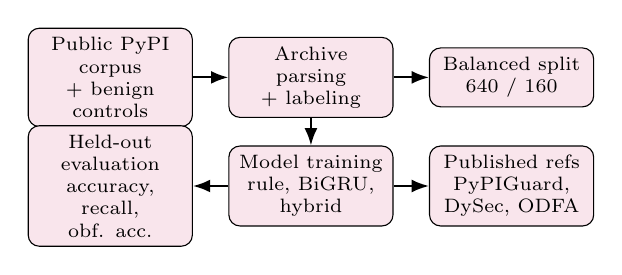
\begin{tikzpicture}[
font=\scriptsize,
node distance=0.35cm and 0.45cm,
box/.style={draw, rounded corners, text width=1.85cm, minimum height=0.58cm, align=center, fill=purple!10},
arrow/.style={-{Latex[length=2.2mm]}, thick}
]
\node[box] (corpus) {Public PyPI corpus\\ + benign controls};
\node[box, right=of corpus] (extract) {Archive parsing\\ + labeling};
\node[box, right=of extract] (split) {Balanced split\\ 640 / 160};
\node[box, below=of extract] (train) {Model training\\ rule, BiGRU, hybrid};
\node[box, left=of train] (eval) {Held-out evaluation\\ accuracy, recall, obf. acc.};
\node[box, right=of train] (compare) {Published refs\\ PyPIGuard, DySec, ODFA};
\draw[arrow] (corpus) -- (extract);
\draw[arrow] (extract) -- (split);
\draw[arrow] (extract) -- (train);
\draw[arrow] (train) -- (eval);
\draw[arrow] (train) -- (compare);
\end{tikzpicture}
}
\caption{Benchmarking flow used to compare VulnAI's learning-based extension with internal baselines and published references.}
\label{fig:benchmark_flow}
\end{figure}

Fig.~\ref{fig:benchmark_flow} shows that the comparison pipeline moves from corpus construction to archive extraction, balanced train-evaluation splitting, model training, held-out measurement, and only then to external comparison, which clarifies that published systems are used as calibrated reference points rather than as same-split direct baselines.

\subsection{Error Analysis}
Deterministic analysis remains attractive for CI because it is transparent, reproducible, fast, and easier to validate during code review. For high-confidence signals such as structured secrets or explicit dangerous constructs, carefully designed rules remain effective and defensible~\cite{meli2019how}. This is why VulnAI treats deterministic scanning as the baseline control.

The literature on propagated vulnerabilities shows that downstream software may reuse or modify vulnerable components in ways that complicate direct detection~\cite{woo2022movery,woo2023v1scan}. At the same time, exploitability work shows that an advisory alone may overstate actual risk in a specific downstream project~\cite{deng2025chainfuzz}. VulnAI therefore reports dependency vulnerabilities as strong triage signals while avoiding unsupported claims about exploitability.

Learning-based models offer a path to better semantic understanding, vulnerability ranking, and malicious intent inference. Works such as VulBERTa and MSIVD indicate that source-code models and LLM-guided training can improve vulnerability detection quality~\cite{hanif2022vulberta,yang2024msivd}. However, the recent SLR by Kaniewski \emph{et al.} highlights substantial heterogeneity in task formulation, input representation, architecture choices, and dataset design across LLM-based vulnerability detection studies, which complicates comparability and reproducibility~\cite{kaniewski2025slr}. VulnAI is therefore better understood as a practical foundation on top of which model-based enrichment can be added selectively.

VulnAI is not claimed to dominate all prior research methods on raw detection accuracy. Instead, its advantage is deployment fit for repository-integrated defense. Compared with MSDT~\cite{tsfaty2023malicious}, which uses deep-learning embeddings and anomaly detection over a large function corpus to identify malicious injections, VulnAI requires no model training, no 600k-scale function dataset, and no clustering pipeline. This makes VulnAI easier to run in CI on ordinary repositories, while still covering a broader set of operational risks such as secrets, dependency CVEs, risky APIs, and state artifacts in addition to suspicious code patterns.

Compared with many LLM-centered vulnerability detection pipelines summarized by Kaniewski \emph{et al.}~\cite{kaniewski2025slr}, VulnAI is narrower in modeling sophistication but stronger in immediate operational simplicity. It is push-aware, owner-aware, report-oriented, and deterministic by default. In other words, the framework is better suited for lightweight GitHub-native triage, whereas LLM-based systems may be more appropriate when higher-cost semantic analysis, localization, or explanation quality is the primary goal.

At the same time, the benchmarked learning-based extension shows that a compact non-LLM architecture can materially improve malicious-package triage quality without adopting a full-scale code model. The best VulnAI BiGRU variant reached 98.75\% accuracy and 100\% malicious recall on the expanded public PyPI benchmark slice. This narrows the gap to specialized malicious-package detectors and suggests that VulnAI can combine deterministic CI controls with selective model-based enrichment when suspicious artifacts warrant deeper review.

\subsection{Limitations}
The current framework has several limitations:
\begin{itemize}
\item it does not prove exploitability of flagged dependency vulnerabilities,
\item it uses changed-file granularity rather than semantic hunk-level reasoning,
\item it relies on pattern-based detection for suspicious code and may miss novel obfuscation,
\item the benchmarked learning-based extension is evaluated on an expanded local slice derived from public package artifacts rather than on an identical split to MalwareBench or live enterprise streams,
\item it does not currently provide anomaly-based function embedding analysis such as MSDT or full LLM-based vulnerability reasoning,
\item cross-paper comparisons remain indicative rather than strictly head-to-head.
\end{itemize}

\section{Conclusion and Future Work}
This paper presented VulnAI, a GitHub-native framework for automated dependency vulnerability analysis and repository risk detection in open-source software projects. The system combines dependency scanning, secret detection, suspicious-code analysis, memory artifact identification, change-aware triage, and owner-aware reporting into a single CI-compatible workflow. The framework is grounded in prior work on GitHub secret leakage, vulnerability propagation in reused components, exploitability validation in supply chains, commit-level security analysis, and learning-based vulnerability detection. In addition, the paper reported an experimental malicious-package detector that achieved 98.75\% accuracy on an expanded public PyPI benchmark slice, showing that compact deep models can complement deterministic repository defense without resorting to LLM-scale infrastructure.

Future work will focus on hunk-level change analysis, reachability-aware dependency validation, SARIF export, and optional LLM-assisted enrichment for suspicious code review. These extensions would improve ranking and semantic coverage while preserving the deterministic core needed for practical deployment.

\bibliographystyle{IEEEtran}
\bibliography{refs}

\end{document}
